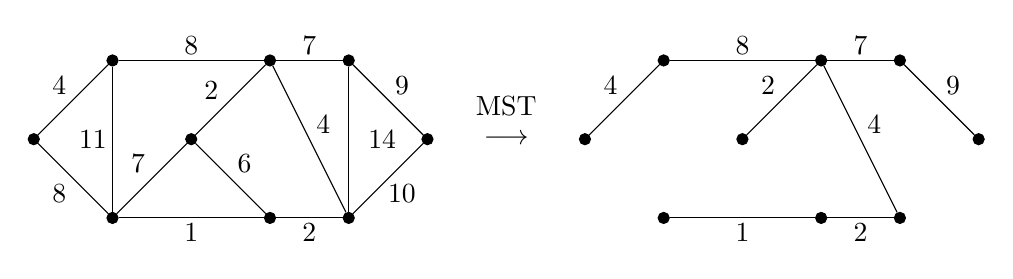
\begin{tikzpicture}[black/.style={circle,draw,fill=black,inner sep=0pt, minimum width=4pt}]
	\foreach \x in {1,3,4}
		\node[black] at (\x,2) (a\x) {};
	\foreach \x in {0,2,5}
		\node[black] at (\x,1) (b\x) {};
	\foreach \x in {1,3,4}
		\node[black] at (\x,0) (c\x) {};
	\draw (a1) -- (a3) node [midway,label={8},yshift=-5] {};
	\draw (a3) -- (a4) node [midway,label={7},yshift=-5] {};
	\draw (c1) -- (c3) node [midway,label=below:{1},yshift=5] {};
	\draw (c3) -- (c4) node [midway,label=below:{2},yshift=5] {};
	\draw (b0) -- (a1) node [midway,label={4},xshift=-5,yshift=-5] {};
	\draw (b0) -- (c1) node [midway,label=below:{8},xshift=-5,yshift=5] {};
	\draw (a1) -- (c1) node [midway,label=left:{11},xshift=5] {};
	\draw (c1) -- (b2) node [midway,label={7},xshift=-5,yshift=-5] {};
	\draw (b2) -- (c3) node [midway,label={6},xshift=5,yshift=-5] {};
	\draw (b2) -- (a3) node [midway,label={2},xshift=-7,yshift=-7] {};
	\draw (a3) -- (c4) node [midway,label={4},xshift=5,yshift=-5] {};
	\draw (a4) -- (b5) node [midway,label={9},xshift=5,yshift=-5] {};
	\draw (c4) -- (b5) node [midway,label=below:{10},xshift=5,yshift=5] {};
	\draw (a4) -- (c4) node [midway,label=right:{14}] {};


	\draw node at (6,1) {$\longrightarrow$};
	\draw[above,yshift=5] node at (6,1) {MST};


	\foreach \x in {8,10,11}
		\node[black] at (\x,2) (aa\x) {};
	\foreach \x in {7,9,12}
		\node[black] at (\x,1) (bb\x) {};
	\foreach \x in {8,10,11}
		\node[black] at (\x,0) (cc\x) {};
	\draw (aa8) -- (aa10) node [midway,label={8},yshift=-5] {};
	\draw (aa10) -- (aa11) node [midway,label={7},yshift=-5] {};
	\draw (cc8) -- (cc10) node [midway,label=below:{1},yshift=5] {};
	\draw (cc10) -- (cc11) node [midway,label=below:{2},yshift=5] {};
	\draw (bb7) -- (aa8) node [midway,label={4},xshift=-5,yshift=-5] {};
	% \draw (bb7) -- (cc8) node [midway,label=below:{8},xshift=-5,yshift=5] {};
	% \draw (aa8) -- (cc8) node [midway,label=left:{11},xshift=5] {};
	% \draw (cc8) -- (bb9) node [midway,label={7},xshift=-5,yshift=-5] {};
	% \draw (bb9) -- (cc10) node [midway,label={6},xshift=5,yshift=-5] {};
	\draw (bb9) -- (aa10) node [midway,label={2},xshift=-5,yshift=-5] {};
	\draw (aa10) -- (cc11) node [midway,label={4},xshift=5,yshift=-5] {};
	\draw (aa11) -- (bb12) node [midway,label={9},xshift=5,yshift=-5] {};
	% \draw (cc11) -- (bb12) node [midway,label=below:{10},xshift=5,yshift=5] {};
	% \draw (aa11) -- (cc11) node [midway,label=right:{14}] {};
\end{tikzpicture}
